\chapter{Pemrograman Berorientasi Objek}

\section{Pengenalan OOP}

Pemrograman Berorientasi Objek (Object-Oriented Programming, disingkat OOP) adalah paradigma pemrograman yang berfokus pada pembuatan \emph{objek} yang merepresentasikan entitas dunia nyata. Setiap objek memiliki \emph{atribut} (data) dan \emph{metode} (perilaku).

Berbeda dengan pendekatan prosedural yang menekankan urutan langkah-langkah (fungsi), OOP menekankan struktur dan hubungan antar objek. Tujuannya adalah agar program lebih mudah dipelihara, diperluas, dan digunakan kembali (reusable).

\subsection*{Konsep Utama OOP}
Beberapa konsep utama dalam OOP adalah:
\begin{enumerate}
    \item \textbf{Kelas (Class)} — cetak biru atau template untuk membuat objek.
    \item \textbf{Objek (Object)} — instance nyata dari sebuah kelas.
    \item \textbf{Atribut (Attribute)} — data atau properti yang dimiliki objek.
    \item \textbf{Metode (Method)} — fungsi yang mendefinisikan perilaku objek.
    \item \textbf{Pewarisan (Inheritance)} — kemampuan kelas untuk mewarisi sifat dari kelas lain.
    \item \textbf{Polimorfisme (Polymorphism)} — kemampuan objek berbeda untuk merespons cara yang sama secara berbeda.
\end{enumerate}

\subsection*{Contoh Perbandingan Pendekatan}
Contoh berikut menunjukkan perbedaan pendekatan prosedural dan OOP dalam konteks yang sama.

\noindent\textbf{Pendekatan Prosedural}
\begin{lstlisting}[style=PythonStyle, caption={Pendekatan Prosedural}]
# Data dan fungsi terpisah
nama = "Rani"
umur = 21

def sapa(nama, umur):
    print(f"Halo {nama}, umur kamu {umur} tahun.")

sapa(nama, umur)
\end{lstlisting}

\noindent\textbf{Pendekatan OOP}
\begin{lstlisting}[style=PythonStyle, caption={Pendekatan Berorientasi Objek}]
# Data dan fungsi disatukan dalam satu kelas
class Orang:
    def __init__(self, nama, umur):
        self.nama = nama
        self.umur = umur

    def sapa(self):
        print(f"Halo {self.nama}, umur kamu {self.umur} tahun.")

o1 = Orang("Rani", 21)
o1.sapa()
\end{lstlisting}

\subsection*{Manfaat OOP}
\begin{itemize}
    \item \textbf{Reusabilitas}: Kelas dapat digunakan kembali dalam berbagai proyek.
    \item \textbf{Modularitas}: Program dapat dibagi menjadi komponen yang lebih kecil dan terpisah.
    \item \textbf{Kemudahan Pemeliharaan}: Perubahan dalam satu bagian program tidak memengaruhi bagian lain secara langsung.
    \item \textbf{Abstraksi dan Enkapsulasi}: Detail implementasi dapat disembunyikan dari pengguna kelas.
\end{itemize}

\subsection*{Ringkasan}
Pendekatan OOP membantu programmer membangun sistem yang lebih terstruktur dengan menyatukan data dan perilaku dalam satu kesatuan logis, yaitu \textbf{objek}. Bab ini menjadi dasar untuk memahami topik-topik berikutnya seperti kelas, atribut, metode, pewarisan, dan polimorfisme.


\section{Kelas dan Objek}

\subsection{Konsep Kelas dan Objek}
Dalam pemrograman berorientasi objek, \textbf{kelas (class)} merupakan \emph{cetak biru} atau \emph{definisi} dari suatu objek.  
Artinya, kelas tidak hanya menjadi rancangan teknis, tetapi juga \textbf{pengertian atau konsep dari objek itu sendiri}.  

Sebagai contoh, jika kita memiliki kelas \texttt{Mahasiswa}, maka kelas tersebut mendefinisikan \emph{apa yang dimaksud dengan seorang mahasiswa} dalam konteks program: atribut apa yang dimiliki, dan perilaku apa yang dapat dilakukan.  
Setiap objek yang dibuat dari kelas tersebut adalah \textbf{realisasi nyata} dari definisi itu.

\begin{center}
\textit{Kelas = definisi atau pengertian dari objek.} \\
\textit{Objek = wujud nyata dari definisi tersebut.}
\end{center}

\begin{lstlisting}[style=PythonStyle, caption={Kelas sebagai Definisi Objek}]
# Definisi kelas Mahasiswa
class Mahasiswa:
    def __init__(self, nama, nim):
        self.nama = nama
        self.nim = nim

# Objek adalah wujud nyata dari definisi di atas
m1 = Mahasiswa("Rani", "A11.2024.0001")
m2 = Mahasiswa("Dani", "A11.2024.0002")

print(m1.nama)  # Rani
print(m2.nama)  # Dani
\end{lstlisting}

Setiap objek memiliki data dan perilakunya sendiri, tetapi semuanya mengikuti definisi yang sama dari kelas yang mendasarinya.  
Dengan demikian, kelas dapat dianggap sebagai \textbf{konsep}, sementara objek adalah \textbf{entitas konkret} di dalam program.

\subsection{Membuat Kelas dan Objek}
Untuk membuat kelas di Python, gunakan kata kunci \texttt{class}. Kelas didefinisikan satu kali, sedangkan objek dapat dibuat berkali-kali dari kelas tersebut.  
Kita juga menggunakan metode khusus \texttt{__init__()} sebagai konstruktor untuk menetapkan nilai awal atribut.

\begin{lstlisting}[style=PythonStyle, caption={Membuat Kelas dan Objek}]
class Mobil:
    def __init__(self, merek, warna):
        self.merek = merek
        self.warna = warna

    def info(self):
        print(f"Mobil {self.merek} berwarna {self.warna}")

# Membuat beberapa objek dari satu definisi kelas
mobil1 = Mobil("Toyota", "Merah")
mobil2 = Mobil("Honda", "Putih")

mobil1.info()
mobil2.info()
\end{lstlisting}

\noindent\textbf{Penjelasan:}
\begin{itemize}
    \item Kelas \texttt{Mobil} adalah \textbf{definisi} tentang apa itu mobil — atribut dan perilakunya.
    \item Objek \texttt{mobil1} dan \texttt{mobil2} adalah \textbf{perwujudan nyata} dari definisi tersebut.
    \item Konstruktor \texttt{\_\_init\_\_()} dipanggil secara otomatis ketika objek baru dibuat.
\end{itemize}

\begin{center}
\begin{tikzpicture}[node distance=2.8cm, every node/.style={font=\small}]
\node (class) [draw, rectangle, rounded corners, fill=gray!15, minimum width=4cm, minimum height=1cm] {Kelas (Definisi): \texttt{Mahasiswa}};
\node (obj1) [below left=0.8cm and 1.3cm of class, draw, rectangle, rounded corners, fill=blue!10, minimum width=3cm, minimum height=1cm] {Objek: Rani};
\node (obj2) [below right=0.8cm and 1.3cm of class, draw, rectangle, rounded corners, fill=blue!10, minimum width=3cm, minimum height=1cm] {Objek: Dani};
\draw[->, thick] (class) -- (obj1);
\draw[->, thick] (class) -- (obj2);
\end{tikzpicture}
\end{center}

\subsection*{Ringkasan}
\begin{itemize}
    \item Kelas adalah \textbf{cetak biru sekaligus definisi} yang mendeskripsikan apa itu objek.
    \item Objek adalah \textbf{wujud nyata} dari definisi tersebut di dalam program.
    \item Semua objek dari kelas yang sama mengikuti struktur dan perilaku yang sama, namun memiliki data sendiri-sendiri.
\end{itemize}


\section{Atribut dan Metode}

\textbf{Atribut} dan \textbf{metode} merupakan dua komponen utama dalam kelas.  
Atribut menyimpan \emph{data atau keadaan} dari objek, sedangkan metode mendefinisikan \emph{perilaku atau aksi} yang dapat dilakukan objek.

Dengan kata lain, atribut menggambarkan \emph{apa yang dimiliki} oleh objek, dan metode menggambarkan \emph{apa yang dapat dilakukan} oleh objek tersebut.

\subsection{Atribut Instans dan Kelas}

Atribut dalam Python terbagi menjadi dua jenis utama:
\begin{enumerate}
    \item \textbf{Atribut Instans} — dimiliki secara unik oleh setiap objek (disimpan di dalam \texttt{self}).
    \item \textbf{Atribut Kelas} — dimiliki bersama oleh semua objek dari kelas yang sama.
\end{enumerate}

\noindent\textbf{Contoh Atribut Instans:}
Atribut ini didefinisikan di dalam konstruktor \texttt{__init__()} dan berbeda untuk setiap objek.

\begin{lstlisting}[style=PythonStyle, caption={Atribut Instans}]
class Mahasiswa:
    def __init__(self, nama, nim):
        self.nama = nama      # atribut instans
        self.nim = nim        # atribut instans

m1 = Mahasiswa("Rani", "A11.2024.0001")
m2 = Mahasiswa("Dani", "A11.2024.0002")

print(m1.nama)  # Rani
print(m2.nama)  # Dani
\end{lstlisting}

Pada contoh di atas, \texttt{m1.nama} dan \texttt{m2.nama} adalah atribut instans yang menyimpan data berbeda pada setiap objek.

\noindent\textbf{Contoh Atribut Kelas:}
Atribut kelas dideklarasikan di luar konstruktor dan nilainya sama untuk semua objek.

\begin{lstlisting}[style=PythonStyle, caption={Atribut Kelas}]
class Mahasiswa:
    universitas = "Pradita University"  # atribut kelas

    def __init__(self, nama, nim):
        self.nama = nama
        self.nim = nim

m1 = Mahasiswa("Rani", "A11.2024.0001")
m2 = Mahasiswa("Dani", "A11.2024.0002")

print(m1.universitas)  # Pradita University
print(m2.universitas)  # Pradita University
\end{lstlisting}

Jika nilai atribut kelas diubah dari nama kelasnya, maka perubahan akan berlaku untuk semua objek.

\begin{lstlisting}[style=PythonStyle, caption={Perubahan Atribut Kelas}]
Mahasiswa.universitas = "Universitas Python"

print(m1.universitas)  # Universitas Python
print(m2.universitas)  # Universitas Python
\end{lstlisting}

\noindent\textbf{Perbedaan Penting:}
\begin{itemize}
    \item Atribut instans: menyimpan data spesifik tiap objek.
    \item Atribut kelas: digunakan bersama oleh semua objek dari kelas tersebut.
\end{itemize}

\subsection{Metode dan \texttt{self}}

Metode adalah fungsi yang didefinisikan di dalam kelas. Metode digunakan untuk mendeskripsikan \textbf{perilaku} dari objek.  
Setiap metode memiliki parameter pertama bernama \texttt{self}, yang mereferensikan objek yang memanggil metode tersebut.

\begin{lstlisting}[style=PythonStyle, caption={Metode dengan self}]
class Mahasiswa:
    def __init__(self, nama, nim):
        self.nama = nama
        self.nim = nim

    def sapa(self):
        print(f"Halo, saya {self.nama} ({self.nim})")

m1 = Mahasiswa("Rani", "A11.2024.0001")
m2 = Mahasiswa("Dani", "A11.2024.0002")

m1.sapa()
m2.sapa()
\end{lstlisting}

\noindent\textbf{Penjelasan:}
\begin{itemize}
    \item \texttt{self} selalu mengacu pada objek yang sedang aktif.
    \item Ketika kita memanggil \texttt{m1.sapa()}, Python secara otomatis meneruskan objek \texttt{m1} sebagai argumen pertama \texttt{self}.
    \item Dengan demikian, setiap metode dapat mengakses atribut milik objek yang memanggilnya.
\end{itemize}

\noindent\textbf{Contoh dengan Perilaku Tambahan:}
\begin{lstlisting}[style=PythonStyle, caption={Metode yang Mengubah Keadaan Objek}]
class Mobil:
    def __init__(self, merek, kecepatan=0):
        self.merek = merek
        self.kecepatan = kecepatan

    def tambah_kecepatan(self, delta):
        self.kecepatan += delta

    def info(self):
        print(f"{self.merek} melaju {self.kecepatan} km/jam")

mobil1 = Mobil("Toyota")
mobil1.tambah_kecepatan(50)
mobil1.info()
\end{lstlisting}

Dalam contoh di atas:
\begin{itemize}
    \item \texttt{tambah_kecepatan()} adalah metode yang mengubah \textbf{keadaan objek}.
    \item \texttt{info()} adalah metode untuk menampilkan \textbf{informasi dari keadaan tersebut}.
\end{itemize}

\subsection*{Hubungan Atribut dan Metode}
Kombinasi atribut dan metode menjadikan setiap objek \emph{hidup} — ia memiliki keadaan (data) dan perilaku (aksi).  
Keduanya tidak terpisahkan karena definisi objek selalu mencakup keduanya:  
\emph{"Apa yang dimiliki" dan "apa yang dapat dilakukan".}

\begin{center}
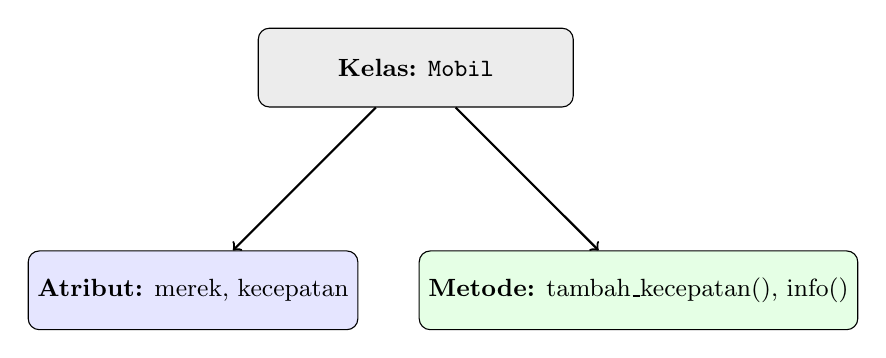
\begin{tikzpicture}[node distance=4cm, every node/.style={font=\small}]
\node (class) [draw, rectangle, rounded corners, fill=gray!15, minimum width=4cm, minimum height=1cm] {\textbf{Kelas:} \texttt{Mobil}};
\node (attr) [below left of=class, draw, rectangle, rounded corners, fill=blue!10, minimum width=3cm, minimum height=1cm] {\textbf{Atribut:} merek, kecepatan};
\node (method) [below right of=class, draw, rectangle, rounded corners, fill=green!10, minimum width=3cm, minimum height=1cm] {\textbf{Metode:} tambah\_kecepatan(), info()};
\draw[->, thick] (class) -- (attr);
\draw[->, thick] (class) -- (method);
\end{tikzpicture}
\end{center}


\subsection*{Ringkasan}
\begin{itemize}
    \item \textbf{Atribut} menyimpan data atau keadaan objek.
    \item \textbf{Metode} mendefinisikan perilaku objek.
    \item \texttt{self} digunakan untuk mengakses atribut dan metode milik objek itu sendiri.
    \item Atribut kelas dimiliki bersama, sedangkan atribut instans spesifik untuk tiap objek.
\end{itemize}

\section{Pewarisan (Inheritance)}

\textbf{Pewarisan (Inheritance)} adalah salah satu konsep inti dalam pemrograman berorientasi objek (OOP).  
Konsep ini memungkinkan sebuah kelas untuk \textbf{mewarisi atribut dan metode dari kelas lain}.  
Dengan pewarisan, kita dapat membuat kelas baru yang mewarisi perilaku dari kelas yang sudah ada tanpa menulis ulang semua kodenya.

\begin{center}
\textit{Tujuan pewarisan adalah untuk memanfaatkan kembali kode dan membangun hierarki kelas yang lebih logis.}
\end{center}

\subsection{Konsep Pewarisan}

Kelas yang diwarisi disebut \textbf{kelas induk (superclass atau parent class)},  
sedangkan kelas yang mewarisi disebut \textbf{kelas turunan (subclass atau child class)}.  
Kelas turunan dapat:
\begin{itemize}
    \item Menggunakan atribut dan metode dari kelas induk.
    \item Menambahkan atribut atau metode baru.
    \item Menimpa (override) metode yang sudah ada untuk perilaku khusus.
\end{itemize}

\noindent\textbf{Contoh Pewarisan Sederhana:}

\begin{lstlisting}[style=PythonStyle, caption={Contoh Pewarisan Dasar}]
# Kelas induk
class Kendaraan:
    def __init__(self, merek):
        self.merek = merek

    def info(self):
        print(f"Kendaraan merek {self.merek}")

# Kelas turunan
class Mobil(Kendaraan):
    def __init__(self, merek, jumlah_pintu):
        self.merek = merek
        self.jumlah_pintu = jumlah_pintu

    def info(self):
        print(f"Mobil {self.merek} dengan {self.jumlah_pintu} pintu")

# Membuat objek
k1 = Kendaraan("Yamaha")
m1 = Mobil("Toyota", 4)

k1.info()
m1.info()
\end{lstlisting}

Kelas \texttt{Mobil} di atas mewarisi struktur dari \texttt{Kendaraan}, tetapi menambahkan atribut baru (\texttt{jumlah\_pintu}) dan menimpa metode \texttt{info()} untuk menampilkan perilaku yang berbeda.

\begin{center}
\begin{tikzpicture}[node distance=2.8cm, every node/.style={font=\small}]
\node (super) [draw, rectangle, rounded corners, fill=gray!15, minimum width=4cm, minimum height=1cm] {Kelas Induk: \texttt{Kendaraan}};
\node (child) [below=1.5cm of super, draw, rectangle, rounded corners, fill=blue!10, minimum width=4cm, minimum height=1cm] {Kelas Turunan: \texttt{Mobil}};
\draw[->, thick] (super) -- (child) node[midway, right] {mewarisi};
\end{tikzpicture}
\end{center}

\noindent\textbf{Manfaat Pewarisan:}
\begin{itemize}
    \item Menghindari duplikasi kode.
    \item Memudahkan perluasan (ekstensi) fungsi program.
    \item Menyusun hubungan hierarkis yang alami antar kelas.
\end{itemize}

\noindent\textbf{Contoh Hierarki Pewarisan Lebih Dalam:}

\begin{lstlisting}[style=PythonStyle, caption={Hierarki Tiga Tingkat}]
class Kendaraan:
    def bergerak(self):
        print("Kendaraan bergerak")

class Mobil(Kendaraan):
    def bergerak(self):
        print("Mobil melaju di jalan")

class MobilBalap(Mobil):
    def bergerak(self):
        print("Mobil balap melaju sangat cepat!")

# Objek dari masing-masing kelas
k = Kendaraan()
m = Mobil()
mb = MobilBalap()

for obj in [k, m, mb]:
    obj.bergerak()
\end{lstlisting}

Kode di atas memperlihatkan konsep pewarisan bertingkat (multi-level inheritance).  
Setiap kelas dapat menimpa metode \texttt{bergerak()} dengan perilaku yang semakin spesifik.

\subsection{Menggunakan \texttt{super()}}

Ketika kelas turunan memiliki konstruktor sendiri, kita sering kali masih ingin memanggil konstruktor dari kelas induk agar atribut dasarnya juga diinisialisasi.  
Untuk itu, Python menyediakan fungsi \texttt{super()}.

\noindent\textbf{Contoh Penggunaan \texttt{super()}:}

\begin{lstlisting}[style=PythonStyle, caption={Menggunakan super() untuk Memanggil Konstruktor Induk}]
class Kendaraan:
    def __init__(self, merek):
        self.merek = merek

class Mobil(Kendaraan):
    def __init__(self, merek, jumlah_pintu):
        super().__init__(merek)   # memanggil konstruktor kelas induk
        self.jumlah_pintu = jumlah_pintu

    def info(self):
        print(f"{self.merek} - {self.jumlah_pintu} pintu")

m1 = Mobil("Honda", 4)
m1.info()
\end{lstlisting}

Tanpa \texttt{super()}, kita harus menulis ulang inisialisasi atribut dari kelas induk, yang berpotensi menyebabkan duplikasi kode.

\textbf{Catatan Penting tentang \texttt{super()}:}
\begin{itemize}
    \item \texttt{super()} digunakan untuk mengakses metode atau konstruktor dari kelas induk.
    \item Umumnya dipakai di dalam metode \texttt{__init__()} agar atribut induk tetap terinisialisasi.
    \item Mendukung pewarisan bertingkat — Python secara otomatis mengikuti urutan hierarki kelas (\textbf{Method Resolution Order, MRO}).
\end{itemize}

\noindent\textbf{Contoh Pewarisan Bertingkat dengan \texttt{super()}:}

\begin{lstlisting}[style=PythonStyle, caption={super() dalam Pewarisan Bertingkat}]
class Kendaraan:
    def __init__(self):
        print("Kendaraan dibuat")

class Mobil(Kendaraan):
    def __init__(self):
        super().__init__()
        print("Mobil dibuat")

class MobilBalap(Mobil):
    def __init__(self):
        super().__init__()
        print("Mobil balap dibuat")

obj = MobilBalap()
\end{lstlisting}

Output:
\begin{lstlisting}[language=bash, caption={Output Program}]
Kendaraan dibuat
Mobil dibuat
Mobil balap dibuat
\end{lstlisting}

\subsection*{Ringkasan}
\begin{itemize}
    \item Pewarisan memungkinkan kelas baru menggunakan ulang kode dari kelas lain.
    \item Kelas induk = sumber definisi, kelas turunan = perluasan atau penyesuaian.
    \item \texttt{super()} digunakan untuk memanggil metode dari kelas induk, biasanya dalam konstruktor.
    \item Pewarisan mendukung hierarki bertingkat dan konsep polimorfisme.
\end{itemize}


\section{Polimorfisme}

\textbf{Polimorfisme (Polymorphism)} berasal dari bahasa Yunani: \emph{poly} berarti banyak, dan \emph{morph} berarti bentuk.  
Dalam konteks OOP, polimorfisme berarti bahwa \textbf{satu antarmuka dapat digunakan untuk berbagai bentuk objek yang berbeda}.  
Setiap objek dapat merespons cara yang sama (\emph{method call}) dengan perilaku yang berbeda-beda.

\begin{center}
\textit{Dengan polimorfisme, objek-objek dari kelas turunan dapat digunakan seolah-olah mereka adalah objek dari kelas induk.}
\end{center}

Polimorfisme membuat kode lebih fleksibel, mudah diperluas, dan tidak perlu diubah setiap kali jenis objek baru ditambahkan.

\subsection{Konsep Polimorfisme dan Overriding}

Polimorfisme biasanya muncul bersama dengan \textbf{pewarisan} dan \textbf{overriding}.  
Overriding berarti kelas turunan menulis ulang (menimpa) metode dari kelas induk untuk memberikan perilaku yang berbeda sesuai konteksnya sendiri.

\textbf{Contoh Sederhana Polimorfisme:}

\begin{lstlisting}[style=PythonStyle, caption={Polimorfisme dengan Overriding}]
class Hewan:
    def suara(self):
        print("Hewan mengeluarkan suara.")

class Kucing(Hewan):
    def suara(self):
        print("Meong")

class Anjing(Hewan):
    def suara(self):
        print("Guk guk")

# Semua objek dapat diperlakukan sama (sebagai Hewan)
hewan_list = [Hewan(), Kucing(), Anjing()]

for h in hewan_list:
    h.suara()
\end{lstlisting}

\begin{lstlisting}[language=bash, caption={Output Program}]
Hewan mengeluarkan suara.
Meong
Guk guk
\end{lstlisting}

Dalam contoh di atas:
\begin{itemize}
    \item Semua kelas (\texttt{Hewan}, \texttt{Kucing}, \texttt{Anjing}) memiliki metode \texttt{suara()}.
    \item Implementasinya berbeda untuk setiap kelas.
    \item Ketika loop \texttt{for h in hewan\_list} dijalankan, Python secara otomatis memanggil versi metode yang sesuai dengan objeknya.
\end{itemize}

\textbf{Polimorfisme Tanpa Pewarisan Langsung (Duck Typing):}

Python mendukung konsep \textbf{duck typing} —  
yaitu bentuk polimorfisme di mana tipe objek tidak perlu sama, selama objek memiliki metode yang dibutuhkan.

\begin{lstlisting}[style=PythonStyle, caption={Contoh Duck Typing}]
class Burung:
    def terbang(self):
        print("Burung terbang di langit.")

class Pesawat:
    def terbang(self):
        print("Pesawat lepas landas di landasan.")

# Fungsi yang menerima objek apa pun yang punya metode terbang()
def uji_terbang(obj):
    obj.terbang()

uji_terbang(Burung())
uji_terbang(Pesawat())
\end{lstlisting}

\begin{lstlisting}[language=bash, caption={Output Program}]
Burung terbang di langit.
Pesawat lepas landas di landasan.
\end{lstlisting}

Konsep ini disebut “duck typing” dari pepatah:
\begin{center}
\textit{“If it walks like a duck and quacks like a duck, it’s probably a duck.”}
\end{center}

Artinya, Python tidak peduli dari kelas mana objek berasal —  
selama objek memiliki metode yang diharapkan, maka objek tersebut dapat digunakan.

\textbf{Polimorfisme dalam Hierarki Kelas:}

\begin{lstlisting}[style=PythonStyle, caption={Hierarki Pewarisan dengan Polimorfisme}]
class Kendaraan:
    def bergerak(self):
        print("Kendaraan bergerak.")

class Mobil(Kendaraan):
    def bergerak(self):
        print("Mobil melaju di jalan.")

class Kapal(Kendaraan):
    def bergerak(self):
        print("Kapal berlayar di laut.")

class Pesawat(Kendaraan):
    def bergerak(self):
        print("Pesawat terbang di udara.")

kendaraan_list = [Mobil(), Kapal(), Pesawat()]

for k in kendaraan_list:
    k.bergerak()
\end{lstlisting}

\begin{lstlisting}[language=bash, caption={Output Program}]
Mobil melaju di jalan.
Kapal berlayar di laut.
Pesawat terbang di udara.
\end{lstlisting}

Setiap objek dapat dipanggil dengan cara yang sama, yaitu \texttt{k.bergerak()},  
namun hasil yang ditampilkan berbeda tergantung jenis objeknya — inilah hakikat dari polimorfisme.

\begin{center}
\begin{tikzpicture}[node distance=1.6cm, every node/.style={font=\small}]
\node (super) [draw, rectangle, rounded corners, fill=gray!15, minimum width=4cm, minimum height=1cm] {Kelas Induk: \texttt{Kendaraan}};
\node (mobil) [below left=1.2cm and 2.0cm of super, draw, rectangle, rounded corners, fill=blue!10, minimum width=3cm, minimum height=1cm] {Kelas Turunan: \texttt{Mobil}};
\node (kapal) [below=1.2cm of super, draw, rectangle, rounded corners, fill=blue!10, minimum width=3cm, minimum height=1cm] {Kelas Turunan: \texttt{Kapal}};
\node (pesawat) [below right=1.2cm and 2.0cm of super, draw, rectangle, rounded corners, fill=blue!10, minimum width=3cm, minimum height=1cm] {Kelas Turunan: \texttt{Pesawat}};
\draw[->, thick] (super) -- (mobil);
\draw[->, thick] (super) -- (kapal);
\draw[->, thick] (super) -- (pesawat);
\end{tikzpicture}
\end{center}

\subsection*{Ringkasan}
\begin{itemize}
    \item Polimorfisme memungkinkan satu metode dipanggil pada berbagai objek dengan hasil yang berbeda.
    \item Overriding terjadi ketika kelas turunan menimpa metode kelas induk.
    \item Python mendukung polimorfisme baik melalui pewarisan maupun \emph{duck typing}.
    \item Dengan polimorfisme, kode menjadi lebih fleksibel, mudah diperluas, dan alami dalam menggambarkan perilaku dunia nyata.
\end{itemize}

\section{Latihan}

Bagian ini berisi latihan praktis untuk memperdalam pemahaman konsep OOP di Python — mencakup kelas, objek, atribut, metode, pewarisan, dan polimorfisme.  
Setiap latihan dirancang agar mahasiswa dapat mempraktikkan konsep secara bertahap, mulai dari dasar hingga penerapan dalam konteks nyata.

\subsection*{Latihan 1: Membuat Kelas dan Objek}
Buat sebuah kelas bernama \texttt{Mahasiswa} dengan ketentuan berikut:
\begin{enumerate}
    \item Memiliki atribut \texttt{nama}, \texttt{nim}, dan \texttt{jurusan}.
    \item Memiliki metode \texttt{tampilkan\_info()} yang menampilkan semua atribut di layar.
    \item Buat minimal dua objek dari kelas tersebut dan panggil metode \texttt{tampilkan\_info()} untuk masing-masing.
\end{enumerate}

\begin{lstlisting}[style=PythonStyle, caption={Contoh keluaran yang diharapkan (tidak harus identik)}]
Nama: Rani
NIM: A11.2024.0001
Jurusan: Informatika

Nama: Dani
NIM: A11.2024.0002
Jurusan: Sistem Informasi
\end{lstlisting}

\subsection*{Latihan 2: Atribut dan Metode}
Kembangkan kelas \texttt{Mahasiswa} sebelumnya dengan:
\begin{enumerate}
    \item Menambahkan atribut kelas bernama \texttt{universitas}.
    \item Membuat metode baru \texttt{ubah\_jurusan(jurusan\_baru)} yang mengubah nilai atribut \texttt{jurusan}.
    \item Panggil metode tersebut dan tampilkan hasil perubahan.
\end{enumerate}

\subsection*{Latihan 3: Pewarisan}
Buat hierarki kelas berikut:
\begin{itemize}
    \item Kelas induk: \texttt{Kendaraan} dengan atribut \texttt{merek} dan metode \texttt{bergerak()}.
    \item Kelas turunan: \texttt{Mobil} dan \texttt{SepedaMotor}, masing-masing menimpa metode \texttt{bergerak()}.
    \item Tambahkan konstruktor di setiap kelas dan panggil konstruktor induk menggunakan \texttt{super()}.
\end{itemize}

\begin{lstlisting}[style=PythonStyle, caption={Contoh penggunaan}]
k1 = Mobil("Toyota")
k2 = SepedaMotor("Honda")

k1.bergerak()
k2.bergerak()
\end{lstlisting}

\begin{lstlisting}[language=bash, caption={Output Program}]
Mobil Toyota melaju di jalan raya.
Sepeda motor Honda berjalan di aspal.
\end{lstlisting}

\subsection*{Latihan 4: Polimorfisme}
Buat fungsi \texttt{uji\_bergerak(kendaraan)} yang menerima objek apa pun yang memiliki metode \texttt{bergerak()}.  
Gunakan kelas-kelas dari latihan sebelumnya (\texttt{Kendaraan}, \texttt{Mobil}, \texttt{SepedaMotor}), dan tambahkan satu kelas baru \texttt{Pesawat} yang juga memiliki metode \texttt{bergerak()}.

\begin{enumerate}
    \item Buat daftar berisi beberapa objek dari kelas berbeda.
    \item Gunakan satu loop untuk memanggil \texttt{bergerak()} pada semuanya.
\end{enumerate}

\begin{lstlisting}[language=bash, caption={Output yang Diharapkan}]
Mobil Toyota melaju di jalan raya.
Sepeda motor Honda berjalan di aspal.
Pesawat Garuda terbang di udara.
\end{lstlisting}

\subsection*{Latihan 5: Studi Kasus Mini — Sistem Geometri Bangun Datar}

Rancang sebuah program kecil untuk mendemonstrasikan seluruh konsep OOP yang telah dipelajari melalui perhitungan luas berbagai bangun datar.

\textbf{Deskripsi:}
\begin{itemize}
    \item Buat kelas induk \texttt{BangunDatar} dengan metode \texttt{luas()}.
    \item Buat kelas turunan \texttt{Persegi}, \texttt{PersegiPanjang}, dan \texttt{Lingkaran} yang menimpa metode \texttt{luas()}.
    \item Tambahkan atribut yang sesuai untuk tiap bangun (misalnya \texttt{sisi}, \texttt{panjang}, \texttt{lebar}, \texttt{jari\_jari}).
    \item Gunakan polimorfisme untuk menghitung luas semua bangun dalam satu loop.
\end{itemize}

\begin{lstlisting}[style=PythonStyle, caption={Contoh Implementasi}]
import math

class BangunDatar:
    def luas(self):
        print("Metode luas() harus dioverride di kelas turunan")

class Persegi(BangunDatar):
    def __init__(self, sisi):
        self.sisi = sisi
    def luas(self):
        return self.sisi * self.sisi

class PersegiPanjang(BangunDatar):
    def __init__(self, panjang, lebar):
        self.panjang = panjang
        self.lebar = lebar
    def luas(self):
        return self.panjang * self.lebar

class Lingkaran(BangunDatar):
    def __init__(self, jari_jari):
        self.jari_jari = jari_jari
    def luas(self):
        return math.pi * self.jari_jari ** 2

# Daftar objek dari berbagai kelas turunan
bangun_list = [
    Persegi(5),
    PersegiPanjang(4, 6),
    Lingkaran(7)
]

# Menghitung luas setiap bangun secara polimorfik
for b in bangun_list:
    print(f"Luas {b.__class__.__name__}: {b.luas():.2f}")
\end{lstlisting}

\begin{lstlisting}[language=bash, caption={Output Program}]
Luas Persegi: 25.00
Luas PersegiPanjang: 24.00
Luas Lingkaran: 153.94
\end{lstlisting}

\textbf{Tujuan:}
\begin{itemize}
    \item Menunjukkan bahwa setiap kelas turunan dapat memiliki perilaku (metode) yang berbeda, meskipun memiliki antarmuka yang sama.
    \item Mempraktikkan penggunaan pewarisan dan overriding dalam konteks yang realistis.
    \item Memahami bagaimana polimorfisme memudahkan pemrosesan banyak objek dalam satu struktur kode yang seragam.
\end{itemize}


\subsection*{Refleksi dan Diskusi}
Setelah menyelesaikan seluruh latihan, jawab pertanyaan berikut:
\begin{enumerate}
    \item Apa perbedaan utama antara atribut kelas dan atribut instans?
    \item Mengapa penggunaan \texttt{super()} penting dalam pewarisan?
    \item Bagaimana polimorfisme membantu membuat kode lebih fleksibel?
    \item Apa manfaat praktis konsep OOP dalam membangun aplikasi dunia nyata?
\end{enumerate}

\section{Ringkasan}
	
Bab ini membahas konsep dasar pemrograman berorientasi objek (OOP) di Python, meliputi kelas, objek, atribut, metode, pewarisan, dan polimorfisme. Setiap bagian menekankan bagaimana kelas berfungsi sebagai cetak biru sekaligus definisi dari objek, bagaimana atribut menyimpan keadaan, serta bagaimana metode mendefinisikan perilaku. Melalui konsep pewarisan dan penggunaan \texttt{super()}, mahasiswa dapat membuat hierarki kelas yang efisien dan menghindari duplikasi kode.

Selain itu, bab ini memperkenalkan polimorfisme sebagai kemampuan berbagai objek untuk merespons perintah yang sama dengan cara yang berbeda. Polimorfisme dan duck typing memberikan fleksibilitas tinggi dalam desain program, memungkinkan pengembang membuat sistem yang mudah diperluas, alami, dan sesuai dengan model dunia nyata. Pemahaman konsep-konsep ini menjadi fondasi penting untuk membangun program Python yang modular, dapat digunakan kembali, dan mudah dirawat.

